\let\negmedspace\undefined
\let\negthickspace\undefined
\documentclass[journal,12pt,onecolumn]{IEEEtran}
\usepackage{cite}
\usepackage{amsmath,amssymb,amsfonts,amsthm}
\usepackage{algorithmic}
\usepackage{graphicx}
\usepackage{textcomp}
\usepackage{tikz}
\usepackage{xcolor}
\usepackage{txfonts}
\usepackage{listings}
\usepackage{enumitem}
\usepackage{mathtools}
\usepackage{gensymb}

\usepackage{tkz-euclide} % loads  TikZ and tkz-base
\usepackage{listings}



\newtheorem{theorem}{Theorem}[section]
\newtheorem{problem}{Problem}
\newtheorem{proposition}{Proposition}[section]
\newtheorem{lemma}{Lemma}[section]
\newtheorem{corollary}[theorem]{Corollary}
\newtheorem{example}{Example}[section]
\newtheorem{definition}[problem]{Definition}
%\newtheorem{thm}{Theorem}[section] 
%\newtheorem{defn}[thm]{Definition}
%\newtheorem{algorithm}{Algorithm}[section]
%\newtheorem{cor}{Corollary}
\newcommand{\BEQA}{\begin{eqnarray}}
\newcommand{\EEQA}{\end{eqnarray}}
\newcommand{\system}[1]{\stackrel{#1}{\rightarrow}}

\newcommand{\define}{\stackrel{\triangle}{=}}
\theoremstyle{remark}
\newtheorem{rem}{Remark}
%\bibliographystyle{ieeetr}
\begin{document}
%
\providecommand{\pr}[1]{\ensuremath{\Pr\left(#1\right)}}
\providecommand{\prt}[2]{\ensuremath{p_{#1}^{\left(#2\right)} }}        % own macro for this question
\providecommand{\qfunc}[1]{\ensuremath{Q\left(#1\right)}}
\providecommand{\sbrak}[1]{\ensuremath{{}\left[#1\right]}}
\providecommand{\lsbrak}[1]{\ensuremath{{}\left[#1\right.}}
\providecommand{\rsbrak}[1]{\ensuremath{{}\left.#1\right]}}
\providecommand{\brak}[1]{\ensuremath{\left(#1\right)}}
\providecommand{\lbrak}[1]{\ensuremath{\left(#1\right.}}
\providecommand{\rbrak}[1]{\ensuremath{\left.#1\right)}}
\providecommand{\cbrak}[1]{\ensuremath{\left\{#1\right\}}}
\providecommand{\lcbrak}[1]{\ensuremath{\left\{#1\right.}}
\providecommand{\rcbrak}[1]{\ensuremath{\left.#1\right\}}}
\newcommand{\sgn}{\mathop{\mathrm{sgn}}}
\providecommand{\abs}[1]{\left\vert#1\right\vert}
\providecommand{\res}[1]{\Res\displaylimits_{#1}} 
\providecommand{\norm}[1]{\left\lVert#1\right\rVert}
%\providecommand{\norm}[1]{\lVert#1\rVert}
\providecommand{\mtx}[1]{\mathbf{#1}}
\providecommand{\mean}[1]{E\left[ #1 \right]}
\providecommand{\cond}[2]{#1\middle|#2}
\providecommand{\fourier}{\overset{\mathcal{F}}{ \rightleftharpoons}}
\newenvironment{amatrix}[1]{%
  \left(\begin{array}{@{}*{#1}{c}|c@{}}
}{%
  \end{array}\right)
}
%\providecommand{\hilbert}{\overset{\mathcal{H}}{ \rightleftharpoons}}
%\providecommand{\system}{\overset{\mathcal{H}}{ \longleftrightarrow}}
	%\newcommand{\solution}[2]{\textbf{Solution:}{#1}}
\newcommand{\solution}{\noindent \textbf{Solution: }}
\newcommand{\cosec}{\,\text{cosec}\,}
\providecommand{\dec}[2]{\ensuremath{\overset{#1}{\underset{#2}{\gtrless}}}}
\newcommand{\myvec}[1]{\ensuremath{\begin{pmatrix}#1\end{pmatrix}}}
\newcommand{\mydet}[1]{\ensuremath{\begin{vmatrix}#1\end{vmatrix}}}
\newcommand{\myaugvec}[2]{\ensuremath{\begin{amatrix}{#1}#2\end{amatrix}}}
\providecommand{\rank}{\text{rank}}
\providecommand{\pr}[1]{\ensuremath{\Pr\left(#1\right)}}
\providecommand{\qfunc}[1]{\ensuremath{Q\left(#1\right)}}
	\newcommand*{\permcomb}[4][0mu]{{{}^{#3}\mkern#1#2_{#4}}}
\newcommand*{\perm}[1][-3mu]{\permcomb[#1]{P}}
\newcommand*{\comb}[1][-1mu]{\permcomb[#1]{C}}
\providecommand{\qfunc}[1]{\ensuremath{Q\left(#1\right)}}
\providecommand{\gauss}[2]{\mathcal{N}\ensuremath{\left(#1,#2\right)}}
\providecommand{\diff}[2]{\ensuremath{\frac{d{#1}}{d{#2}}}}
\providecommand{\myceil}[1]{\left \lceil #1 \right \rceil }
\newcommand\figref{Fig.~\ref}
\newcommand\tabref{Table~\ref}
\newcommand{\sinc}{\,\text{sinc}\,}
\newcommand{\rect}{\,\text{rect}\,}
%%
%	%\newcommand{\solution}[2]{\textbf{Solution:}{#1}}
%\newcommand{\solution}{\noindent \textbf{Solution: }}
%\newcommand{\cosec}{\,\text{cosec}\,}
%\numberwithin{equation}{section}
%\numberwithin{equation}{subsection}
%\numberwithin{problem}{section}
%\numberwithin{definition}{section}
%\makeatletter
%\@addtoreset{figure}{problem}
%\makeatother

%\let\StandardTheFigure\thefigure
\let\vec\mathbf

\bibliographystyle{IEEEtran}





\bigskip


\title{Gate 2023\_nm\_33}
\author{Karyampudi Meghana Sai\\ EE23BTECH11031}

\maketitle

For a regular sinusoidal wave propagating in deep water having wave height of 3.5 m and wave period of 9 s, the wave steepness is \underline{\hspace{1cm}} (round off to three decimal places).
\hfill Gate 2023 NM 33

\solution

\begin{table}[h]
 	\centering
 	\resizebox{6 cm}{!}{
 		\begin{tabular}{|c|c|c|}
	\hline
	\textbf{Symbol} & \textbf{Value} &
	\textbf{Description}\\[6pt]
	\hline
	$H$ &  $3.5m$ & wave height\\[6pt]
	\hline 
	$T$ & $9s$ & wave period\\[6pt]
	\hline
	$S$ & $ ? $ & wave steepness\\[6pt]
	\hline
	$L$ & $  $ & wave length\\[6pt]
	\hline
\end{tabular}

 	}
 	\vspace{6 pt}
 	\caption{Input Parameters}
 	\label{} 
 \end{table} 
 
 \begin{figure}[h!]
    \centering
    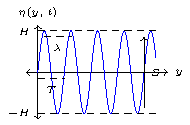
\includegraphics[width=\columnwidth]{figs/figs1.pdf}
    \caption{Sinusoidal wave}
    \label{fig:}
\end{figure} 

\begin{align}
S&=\frac{H}{\lambda} \label{eq:gatenm33eq1}
\end{align}
 Deriving the formula for wavelength of deep water wave:\\

Let's start with the linearized shallow water wave equation.\\
\begin{align}
\frac{\partial^2 \eta}{\partial t^2}=g \frac{\partial \eta}{\partial y}\label{eq:gatenm33eq2}\\
\eta = A\sin(ky - \omega t) \label{eq:gatenm33eq3} \\
\frac{\partial^2 \eta}{\partial t^2} = -(\omega)^2 A\sin(ky - \omega t) \label{eq:gatenm33eq4}
\end{align}
For deep water waves:\\ 
\begin{align}
\frac{\partial \eta}{\partial y} &\approx -k\eta \label{eq:gatenm33eq5}
\end{align}
Using the equation \eqref{eq:gatenm33eq2}.
\begin{align}
\frac{\partial^2 \eta}{\partial t^2}&=-gk\eta \label{eq:gatenm33eq6}\\
&=-gk A\sin(ky - \omega t) \label{eq:gatenm33eq7}
\end{align}
where, k is wave number. \\

Comparing equations \eqref{eq:gatenm33eq4} and \eqref{eq:gatenm33eq7},\\
\begin{align}
\omega^2 &= gk \label{eq:gatenm33eq8} \\
\omega &= \frac{2 \pi}{T} \label{eq:gatenm33eq9} \\
k &= \frac{2 \pi}{\lambda} \label{eq:gatenm33eq10} \\
\lambda &= \frac{g \cdot T^2}{2 \pi} \label{eq:gatenm33eq11}
\end{align}
Substituting numericals,\\
\begin{align}
\lambda&=\frac{g \cdot T^2}{2\pi}\\ 
&=\frac{9.81 \brak{9}^2}{2\pi}\\ 
&=126.53m 
\end{align}
Using the equation \eqref{eq:gatenm33eq1}.\\
\begin{align}
S&=\frac{3.5}{126.53}\\ 
&=0.028 
\end{align}
\begin{figure}[h]
    \centering
    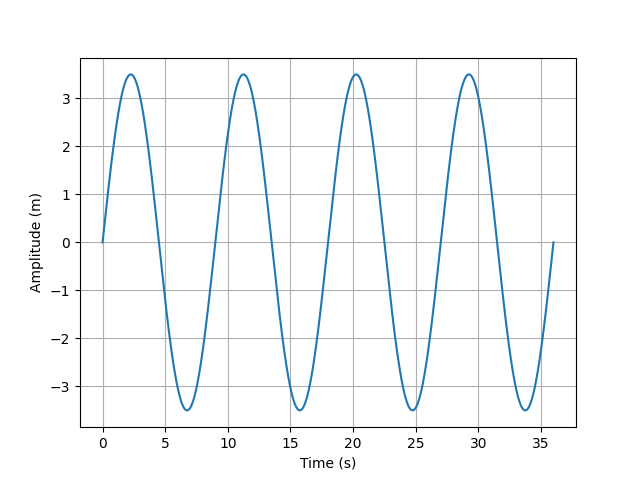
\includegraphics[width=\columnwidth]{figs/plot.png}
    \caption{Sinusoidal wave}
    \label{fig:}
\end{figure} 

\end{document}


